% Chapter: Reinforcement Learning and the Curse of Dimensionality
% Covers complexity results and structural conditions for tractability
% Primary references: Chow-Tsitsiklis (1989), Du et al. (2021), Liu et al. (2022), Lu et al. (2025)

\section{Reinforcement Learning and the Curse of Dimensionality}
\label{sec:curse_of_dimensionality}

\subsection{The Foundational Barrier}
\label{sec:foundational_barrier}

Exact solution methods must visit every state, and the number of states grows exponentially in the problem's natural dimension. With $d$ state variables each taking $n$ discrete values, the state space has $n^d$ elements and value iteration requires $O(n^{2d} \cdot |\mathcal{A}|)$ time per sweep.\footnote{The term ``curse of dimensionality'' is due to \citet{Bellman1957}.} At $d = 10$ and $n = 100$, this exceeds $10^{20}$ operations per sweep.

The theoretical foundations of this barrier were established through a sequence of results in computational complexity. \citet{papadimitriou1987} proved that computing an optimal policy for finite-horizon MDPs is P-complete, placing it among the hardest problems solvable in polynomial time. For infinite-horizon discounted MDPs, they showed that policy iteration terminates in polynomial time, but the polynomial depends on the number of states and actions, which may themselves be exponential in the natural problem dimension.

The decisive complexity result for continuous-state MDPs comes from \citet{chow1989complexity}. Consider the class of discounted MDPs with $d_s$-dimensional continuous state spaces and $d_a$-dimensional continuous action spaces, where the transition density and reward function are Lipschitz continuous. The computational problem is to compute an $\epsilon$-accurate approximation of the optimal value function from evaluations of the reward function and transition density. \citeauthor{chow1989complexity} characterize the worst-case complexity of this problem for deterministic algorithms:

\begin{theorem}[Chow-Tsitsiklis, 1989]
\label{thm:chow_tsitsiklis}
For the class of Lipschitz-continuous discounted MDPs with $d_s$-dimensional states, $d_a$-dimensional actions, and discount factor $\gamma$, the worst-case computational complexity of computing an $\epsilon$-approximation of the optimal value function by any deterministic algorithm with access to function evaluations of the reward and transition density is
\begin{equation}
\Theta\left( \left( \frac{1}{(1-\gamma)^2\,\epsilon} \right)^{2d_s + d_a} \right).
\end{equation}
\end{theorem}

This result has two implications. The upper bound shows that backward induction on uniform discretization grids attains the exponent $2d_s + d_a$; no cleverer deterministic scheme can improve on simple grids by more than constant and logarithmic factors. The lower bound proves that no deterministic algorithm can do better without additional structural assumptions. For a ten-dimensional state space with five-dimensional actions, achieving $\epsilon = 0.01$ accuracy already requires on the order of $10^{50}$ operations from the $\epsilon$-exponent alone, clearly infeasible.

The exponent $2d_s + d_a$ admits a heuristic decomposition into the three numerical subproblems nested in the Bellman operator \citep{rust1996numerical}. Maximizing over the action space contributes $\Theta(\epsilon^{-d_a})$, integrating over the transition density contributes $\Theta(\epsilon^{-d_s})$, and approximating the value function over the state space contributes another $\Theta(\epsilon^{-d_s})$; the complexity bound is the product of the three. The result holds for continuous-action problems, deterministic algorithms, and worst-case complexity, and each of these three qualifications marks an escape route, most notably the random Bellman operators discussed below.

This complexity result extends the work of \citet{traub1988} on information-based complexity, which established similar exponential lower bounds for multivariate integration and function approximation. The connection is direct. Computing expected values under the Bellman operator involves integrating over the transition density, inheriting the curse from numerical integration. \citeauthor{traub1988} showed that for functions in standard Sobolev spaces, no integration method can achieve error $\epsilon$ with fewer than $\Theta(\epsilon^{-d})$ function evaluations. The MDP problem compounds this with the need to solve a fixed-point equation.

\citet{rust1996numerical} surveys these computational barriers in the context of structural econometric estimation of dynamic discrete choice models. The nested fixed-point algorithm (NFXP) requires solving the Bellman equation to compute choice probabilities at each parameter guess, making the curse of dimensionality a binding constraint on the complexity of estimable models.\footnote{This limitation motivated the development of conditional choice probability methods \citep{HotzMiller1993} and simulation-based estimators that avoid full solution of the dynamic program. \citet{rust1997randomization} showed that a random Bellman operator breaks the curse of dimensionality for discrete-choice MDPs, exploiting the fact that randomization breaks the curse of multivariate integration. \citet{bray2022comment} shows that this class of dynamic programs is limited, in that it requires all but a vanishingly small fraction of the state variables to behave arbitrarily similarly to i.i.d.\ uniform random variables.}


\subsection{Breaking the Curse: Three Pathways}
\label{sec:breaking_curse}

Recent theoretical work has identified three distinct structural conditions under which the curse of dimensionality can be circumvented: bilinear structure in the Bellman error, smoothness exploitable by neural networks, and factorization arising from weak coupling.

\subsubsection{Bilinear Structure}

\citet{du2021} introduce the Bilinear Class framework, which unifies and extends prior structural conditions for sample-efficient reinforcement learning. The unifying observation is that many tractable RL settings share a common algebraic property, namely that the Bellman error can be written as a bilinear form.

\begin{definition}[Bilinear Class, Du et al. 2021]
\label{def:bilinear_class}
Consider an MDP $M$, a hypothesis class $\mathcal{H}$, a discrepancy function $\ell_f$, and a set of estimation policies $\Pi_{\text{est}}$. The tuple $(\mathcal{H}, \ell_f, \Pi_{\text{est}}, M)$ is a Bilinear Class if $\mathcal{H}$ is realizable in $M$ and there exist functions $W_h: \mathcal{H} \to \mathcal{V}$ and $X_h: \mathcal{H} \to \mathcal{V}$ for some Hilbert space $\mathcal{V}$ such that for all $f \in \mathcal{H}$ and $h \in [H]$:
\begin{enumerate}
\item The Bellman error decomposes as $\mathbb{E}_{a_{0:h} \sim \pi_f}[Q_{h,f}(s_h, a_h) - r_h - V_{h+1,f}(s_{h+1})] = \langle W_h(f) - W_h(f^*), X_h(f) \rangle$.
\item The discrepancy measure permits estimation. For any $g \in \mathcal{H}$, $|\mathbb{E}_{a_{0:h-1} \sim \pi_f, a_h \sim \pi_{\text{est}}}[\ell_f(o_h, g)]| = |\langle W_h(g) - W_h(f^*), X_h(f) \rangle|$.
\end{enumerate}
\end{definition}

The bilinear structure enables a key computational advantage. Data collected under one hypothesis can be reused to estimate the Bellman error for all hypotheses in the class simultaneously, analogous to uniform convergence in supervised learning. The resulting algorithm, BiLin-UCB, achieves polynomial sample complexity:

\begin{theorem}[Du et al. 2021]
\label{thm:bilinear_sample}
For any Bilinear Class with hypothesis class $\mathcal{H}$ and inherent dimension $d$, there exists an algorithm that returns an $\epsilon$-optimal policy using $\tilde{O}(d^3 H^4 / \epsilon^2)$ samples, where $H$ is the horizon.
\end{theorem}

The Bilinear Class framework subsumes several previously studied settings, including tabular MDPs, linear MDPs \citep{jin2020}, linear mixture MDPs \citep{AyoubVTR2020}, linear Bellman complete models \citep{zanette2020}, and factored MDPs \citep{kearns1999}. It also introduces new tractable settings, including the Linear $Q^*/V^*$ model where both the optimal Q-function and V-function are linear in known features. The unifying observation is that low Bellman rank (the dimension of the bilinear factorization) implies polynomial learnability.\footnote{The Bilinear Class is related to but distinct from the Bellman Eluder dimension of \citet{jin2021}. Neither framework strictly contains the other; they capture different structural properties that enable efficient learning.}


\subsubsection{Smoothness and Neural Function Approximation}

The second pathway exploits smoothness of the value function, which neural networks can approximate efficiently. \citet{liu2022deep} analyze deep Q-learning with $\epsilon$-greedy exploration, characterizing when neural function approximation provably works beyond the linear regime.

The key assumption is that the optimal Q-function lies in a Besov space $\mathcal{B}^{\alpha}_{p,q}(\mathcal{X})$, where $\alpha > 0$ is the smoothness parameter. Besov spaces generalize Sobolev and H\"{o}lder spaces, allowing for spatially inhomogeneous smoothness with spikes and jumps. The smoothness parameter $\alpha$ controls the approximation rate, with smoother functions (larger $\alpha$) admitting more efficient approximation.

\begin{assumption}[Bellman Smoothness, Liu et al. 2022]
\label{ass:bellman_smoothness}
Let $\tilde{R}$ be a fixed constant. Define $\mathcal{B}_{\tilde{R}} = \{f \in \mathcal{B}^{\alpha}_{p,q}(\mathcal{X}): \|f\|_{\mathcal{B}} \leq \tilde{R}\}$. For any $h \in [H]$ and $Q: \mathcal{S} \times \mathcal{A} \to [0, H]$, the Bellman operator satisfies $T^*_h Q \in \mathcal{B}_{\tilde{R}}$.
\end{assumption}

Under this assumption, \citeauthor{liu2022deep} prove that value iteration with deep ReLU networks achieves sublinear regret:

\begin{theorem}[Liu et al. 2022]
\label{thm:deep_rl_regret}
Under Assumption~\ref{ass:bellman_smoothness} with smoothness $\alpha > d(1/p - 1/4)_+$, value iteration via deep ReLU networks with depth $L = O(\log T)$ and width $m = \tilde{O}(T^{d/(2\alpha + d)})$ achieves regret
\begin{equation}
\text{Regret}(T) = \tilde{O}\left( T^{\frac{\alpha K + (\alpha + d)(K+2)}{(2\alpha + d)(K+2)}} \right),
\end{equation}
where $K \in [1, H]$ is an MDP-dependent constant reflecting the exploration difficulty.
\end{theorem}

The regret bound improves with smoothness. As $\alpha \to \infty$, the exponent approaches $(K+1)/(K+2)$, matching the $\epsilon$-greedy contextual bandit rate. For the Barron space (two-layer networks), width $m = \Omega(\sqrt{T})$ suffices, and the bound becomes independent of the ambient dimension $d$, avoiding the curse for sufficiently smooth functions.

The mechanism is that smooth functions can be approximated by neural networks with polynomially many parameters in the accuracy $\epsilon$, rather than the exponential scaling that generic Lipschitz functions require. The curse shifts from state-space size to the smoothness-to-dimension ratio $\alpha/d$; if the target function is sufficiently smooth relative to the dimension, neural approximation breaks the exponential barrier.


\subsubsection{Factorization and Weak Coupling}

The third pathway exploits structural sparsity in the transition dynamics. \citet{lu2025} study factored MDPs where the state vector $s = (s_1, \ldots, s_n)$ consists of $n$ components, and transitions factorize across components:
\begin{equation}
P(s'|s, a) = \prod_{i=1}^{n} P_i(s'_i | s_{\text{pa}(i)}, a),
\end{equation}
where $\text{pa}(i) \subseteq [n]$ denotes the parent set of component $i$. In an exactly factored MDP, each component's next value depends only on a small subset of current components, encoded in a directed graph.

The challenge is that exact factorization rarely holds in practice. \citeauthor{lu2025} extend the theory to approximate factorization, where the true transition kernel $P$ is close to a factored kernel $\tilde{P}$:
\begin{equation}
\Delta_P := \max_{(s,a)} \left\| P(\cdot|s,a) - \tilde{P}(\cdot|s,a) \right\|_{\text{TV}} \leq \delta,
\end{equation}
for some coupling error $\delta \ll 1$. Formally, weak coupling, a common property of networked systems, implies approximate factorization.

\begin{definition}[Weak Coupling]
An MDP exhibits weak coupling if the transition of each state component $s_i$ depends strongly on a small set of parents $\text{pa}(i)$ and only weakly on the remaining components. Formally, the coupling error $\Delta_P$ is small.
\end{definition}

Under approximate factorization, \citeauthor{lu2025} develop two algorithms with polynomial sample complexity:

\begin{theorem}[Lu et al. 2025]
\label{thm:factored_complexity}
For an MDP with $n$ state components, horizon $H$, and coupling error $\Delta_P \leq \delta$, the model-based algorithm achieves $\epsilon$-optimal policy with sample complexity
\begin{equation}
\tilde{O}\left( \frac{|\mathcal{S}_{\text{loc}}|^2 \cdot |\mathcal{A}| \cdot H^4}{\epsilon^2} \right),
\end{equation}
where $|\mathcal{S}_{\text{loc}}|$ is the size of the local state space (determined by the maximum parent set size), rather than the full state space $|\mathcal{S}| = \prod_i |\mathcal{S}_i|$.
\end{theorem}

The exponential dependence on dimension is replaced by polynomial dependence on the local structure. For a system with $n = 100$ components, each with 10 states and parent sets of size 3, the local complexity is $10^3 = 1000$ rather than $10^{100}$.

The practical implication is that networked systems, such as supply chains, power grids, and multi-agent coordination problems, are often amenable to RL methods that exploit the factored structure, even when exact independence does not hold. The coupling error $\Delta_P$ serves as a regularization parameter, where smaller coupling yields faster learning, while the algorithms remain consistent even with moderate coupling.


\subsection{Simulation Study: Wind Farm Storage Control}
\label{sec:wind_farm_simulation}

The barrier of Theorem~\ref{thm:chow_tsitsiklis} and the structural escape routes of Section~\ref{sec:breaking_curse} can both be exhibited in a single control problem, a wind farm with battery storage adapted from the scaling experiment in \citet{lu2025}. Each hour the operator chooses a charge or discharge rate $a_t \in [-20, 20]$ kW, facing stochastic wind generation, spot prices, and demand, over a finite horizon of $H = 24$ hours with discount factor $\gamma = 0.95$. The base state ($d = 3$) is $s_t = (w_t, p_t, c_t)$, where $w_t \in [0, 100]$ is wind generation (kW), $p_t \in [0, 1]$ is the spot price (\$/kWh), and $c_t \in [0, 50]$ is the battery state of charge (kWh); scaling experiments append auxiliary state variables $x_t^{(4)}, \ldots, x_t^{(d)} \in [0, 1]$ that follow AR(1) processes weakly coupled to wind. Transitions are
\begin{align}
w_{t+1} &= 0.7 w_t + \epsilon_t^w, \quad \epsilon_t^w \sim \mathcal{N}(30, 25), \\
p_{t+1} &= 0.6 p_t + 0.05 (w_t / 100) + \epsilon_t^p, \quad \epsilon_t^p \sim \mathcal{N}(0.4, 0.01), \\
c_{t+1} &= c_t + 0.9 a_t, \\
x_{t+1}^{(i)} &= 0.8 x_t^{(i)} + 0.01(w_t/100 - 0.5) + 0.1 + \epsilon_t^{(i)}, \quad \epsilon_t^{(i)} \sim \mathcal{N}(0, 0.0025),
\end{align}
with all variables clipped to their bounds, and the reward is
\begin{equation}
r(s_t, a_t) = p_t \cdot \min(w_t + a_t, D_t) - 0.01 c_t - 5 \cdot \max(0, D_t - w_t - a_t),
\end{equation}
where demand $D_t \sim \text{Poisson}(50 + 10 \sin(2\pi t / 24))$ follows a diurnal pattern. The reward depends only on the base state, so the auxiliary dimensions are payoff-irrelevant yet inflate the state space that any tabular method must enumerate. Four solution methods run at each $d \in \{3, 4, 5, 6\}$. Tabular DP discretizes each dimension into 7 bins and solves by backward induction with Monte Carlo integration over transitions, a benchmark under coarse discretization rather than an exact optimum, granted a 10 minute budget per dimension. Factored RL runs Q-learning with one Q-table per state dimension, aggregated additively; it is given the identity of the three reward-relevant dimensions in advance, so it instantiates the known-structure premise of factored MDPs rather than the algorithms of \citet{lu2025}. DQN is a standard deep Q-network with experience replay and a target network, illustrating the neural function-approximation pathway rather than the specific algorithm analyzed by \citet{liu2022deep}. Linear AC is an actor-critic with linear value and policy functions in polynomial features (intercept, linear, squared, and pairwise cross terms), illustrating the linear function-approximation pathway rather than the BiLin-UCB algorithm of Theorem~\ref{thm:bilinear_sample}. The three RL implementations are illustrative analogies to the three pathways of Section~\ref{sec:breaking_curse}, not implementations of the cited algorithms.\footnote{All methods share the same 11-point action grid. RL methods train for 3{,}000 episodes per seed across 10 seeds; DP uses 20 Monte Carlo samples per state-action pair with a fixed integration seed. Policies are evaluated greedily over 50 episodes on a common evaluation environment (seed 99), so all methods face the same shock sequences. Factored RL uses 30 bins per dimension, learning rate 0.2, and exploration rate 0.2. DQN uses two hidden layers of 128 units, learning rate $5 \times 10^{-4}$, a replay buffer of 10{,}000 transitions, batch size 64, target updates every 100 steps, and $\epsilon$-greedy exploration decaying from 0.3 to 0.01. Linear AC uses actor and critic learning rates of 0.02 and 0.08.}

Table~\ref{tab:curse_results} reports average returns and Figure~\ref{fig:curse_scaling} reports computation times. Tabular DP completes at $d = 3$ (36.7 seconds) and $d = 4$ (317.5 seconds) and exhausts its budget at $d \geq 5$; the exponential fit through its completed runs grows by a factor of 8.6 per added dimension, implying roughly 45.7 minutes at $d = 5$ and 6.6 hours at $d = 6$. The three RL methods train in under a minute per seed at every dimension. Where DP completes, DQN reaches within one percent of the DP return, Factored RL sits two to three percent below it, and Linear AC attains DP-level returns on some seeds while collapsing to substantially worse policies on others, visible in its standard errors. The ranking is unchanged at $d = 5$ and $d = 6$ where DP is intractable. The cost profiles are consistent with the polynomial-complexity scaling predicted by the structural results of Section~\ref{sec:breaking_curse}, with the caveat that the cheapest method is also the least reliable.

\begin{figure}[htbp]
\centering
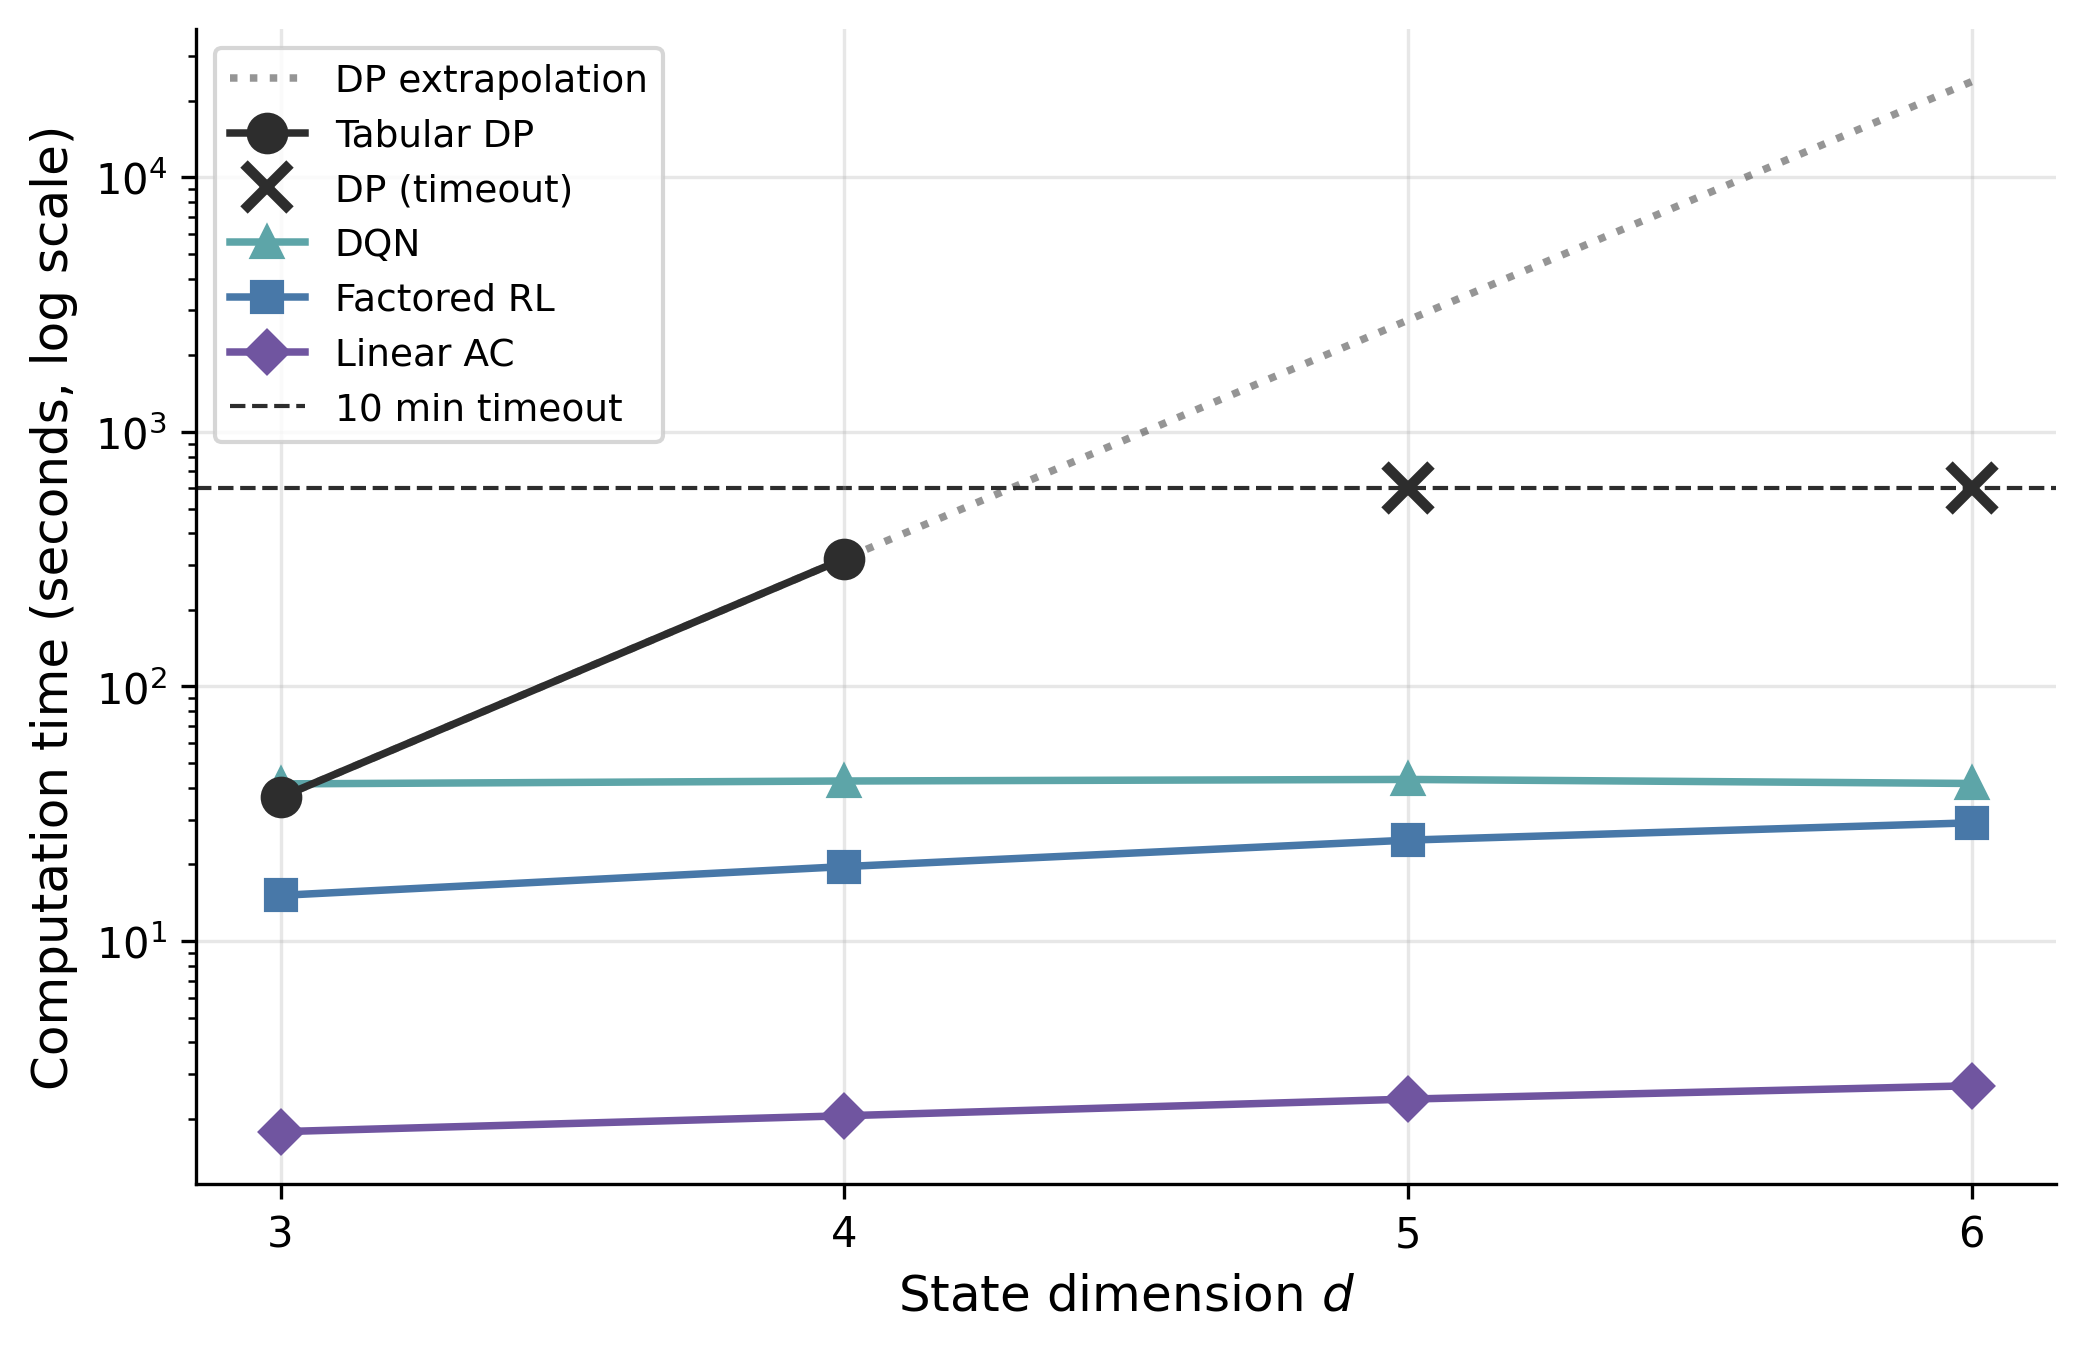
\includegraphics[width=0.7\textwidth]{../ch03_theory/sims/wind_farm_curse_study_times.png}
\caption{Computation time versus state dimension on a log scale. Circles trace completed tabular DP runs and crosses mark runs stopped at the 10 minute budget (dashed reference line); the dotted line extrapolates the exponential fit through the completed DP runs. RL curves show mean training time per seed over 10 seeds.}
\label{fig:curse_scaling}
\end{figure}

\begin{table}[htbp]
\centering
\caption{Average return per episode (\$/day) by method and state dimension. RL cells are mean $\pm$ standard error over 10 training seeds, each evaluated over 50 episodes with common random shocks; the DP row is a single deterministic solve, with TIMEOUT marking dimensions where backward induction exceeded its 10 minute budget. Rows ordered by mean return at $d = 3$.}
\label{tab:curse_results}
\begin{tabular}{lcccc}
\toprule
Method & $d=3$ & $d=4$ & $d=5$ & $d=6$ \\
\midrule
Tabular DP & 1110 & 1113 & TIMEOUT & TIMEOUT \\
DQN & 1108 $\pm$ 0.4 & 1107 $\pm$ 0.7 & 1107 $\pm$ 0.2 & 1100 $\pm$ 0.4 \\
Factored RL & 1091 $\pm$ 4.2 & 1083 $\pm$ 4.1 & 1094 $\pm$ 1.8 & 1084 $\pm$ 4.9 \\
Linear AC & 1002 $\pm$ 29.4 & 1016 $\pm$ 33.9 & 1023 $\pm$ 25.4 & 1009 $\pm$ 30.7 \\
\bottomrule
\end{tabular}

\end{table}
